\chapter{Formal Analysis}
	In this chapter we provide a formal modeling of a restricted part of the system. In particular we modeled:
	\begin{itemize}
		\item selection processes structure;
		\item applications and withdrawals to internship advice (using Alloy 6 temporal operators).
	\end{itemize}
	
	To describe the passing of time (especially in temporal simulations) we built a tiny Alloy \emph{calendar}, which is basically a path of \CommentSty{date} linked each other by means of the relation \CommentSty{yesterday}:
	\begin{center}
		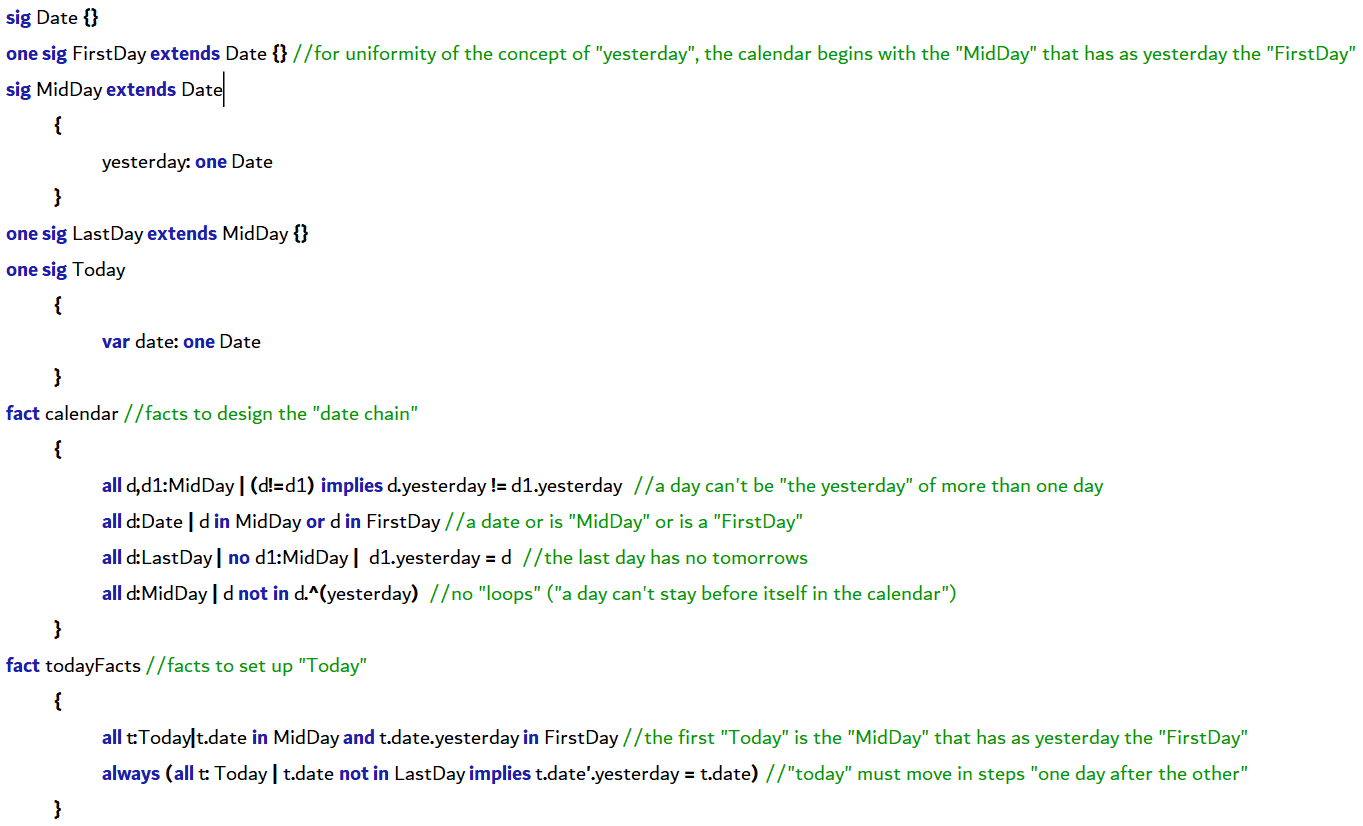
\includegraphics{calendarModel.png}
	\end{center}
	
	Then, What will be generated is a "path of dates" that represents the calendar and \CommentSty{Today} must "move" day-by-day following the calendar structure:
	\begin{center}
		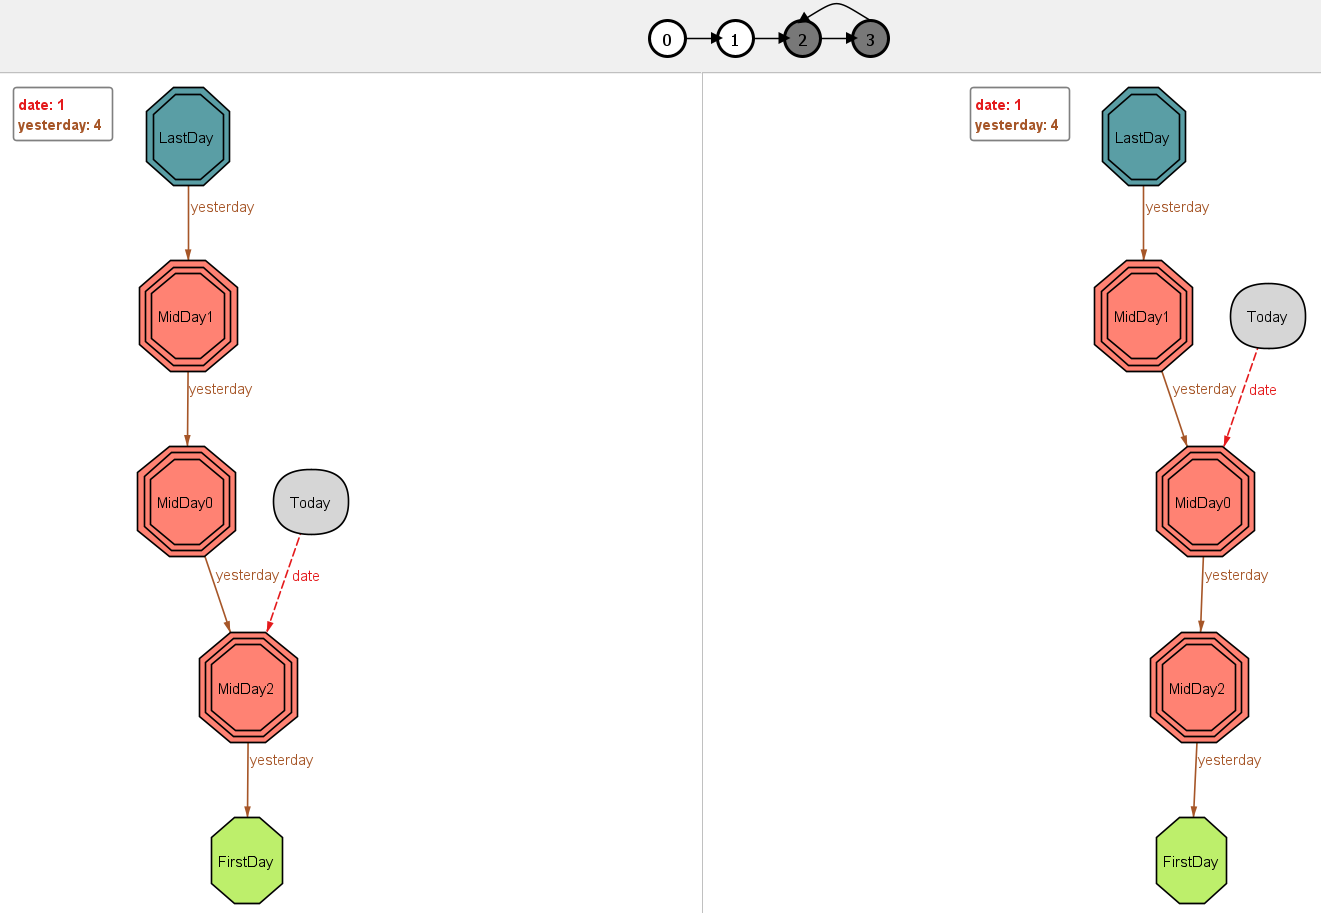
\includegraphics{calendar1.png}
	\end{center}
	\begin{center}
		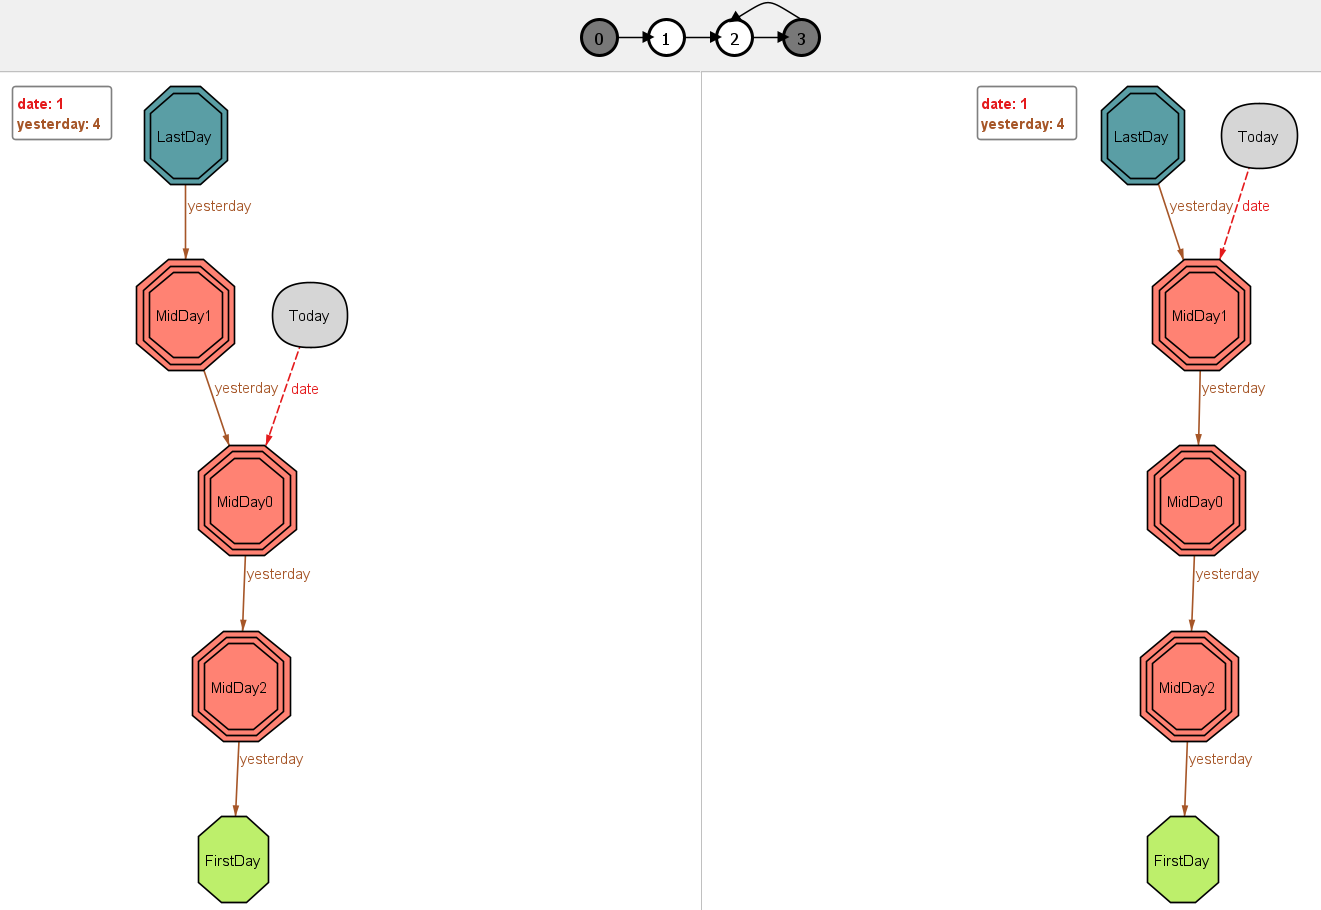
\includegraphics{calendar2.png}
	\end{center}
	
	\section{Applications and withdrawals simulation (Alloy 6 temporal simulation)}
		We modeled a simplified version of the sub-part of the system related to students applications to internship advice. Several parts were omitted in order to highlight what we believed were the most interesting constraints, such as the fact that companies have to accept students applications or the invitation mechanism:
		\begin{center}
			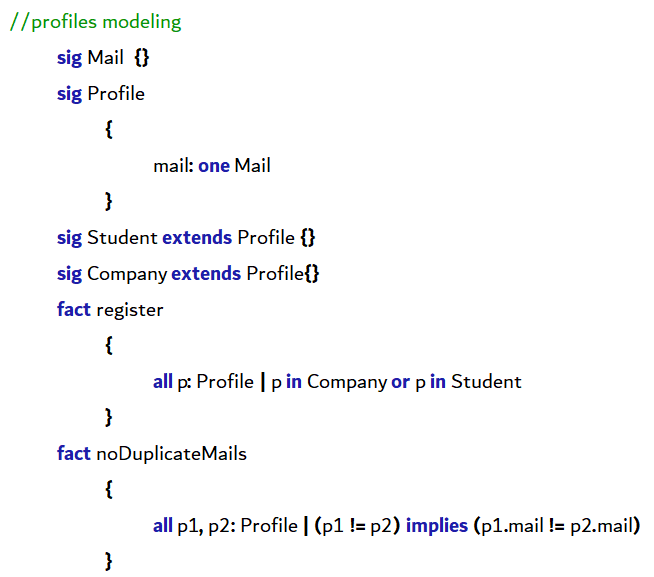
\includegraphics{model1-1.png}
		\end{center}
		\begin{center}
			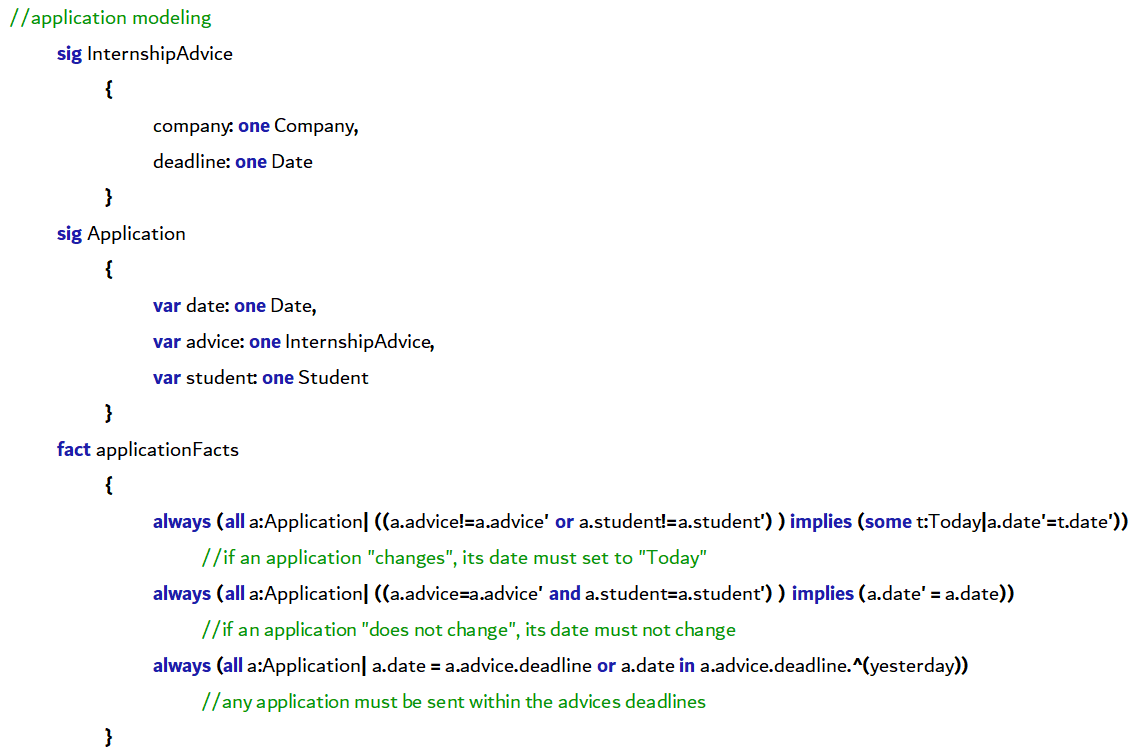
\includegraphics{model1-2.png}
		\end{center}
		By setting up a quite self-explainable predicate to show worlds are trades that can show clearly the expected behavior of the system:
		\begin{center}
			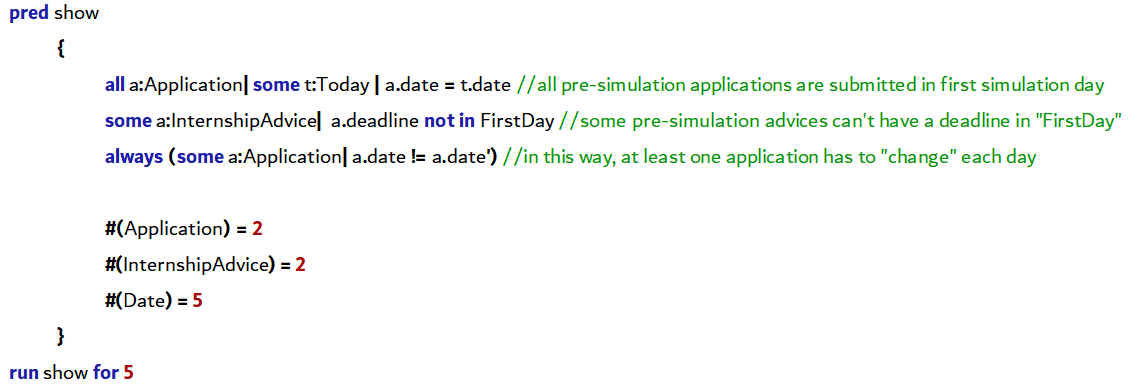
\includegraphics{model1-3.png}
		\end{center}
		we can simulate a classic scenario where students sends applications for available advice within deadlines:
		\begin{center}
			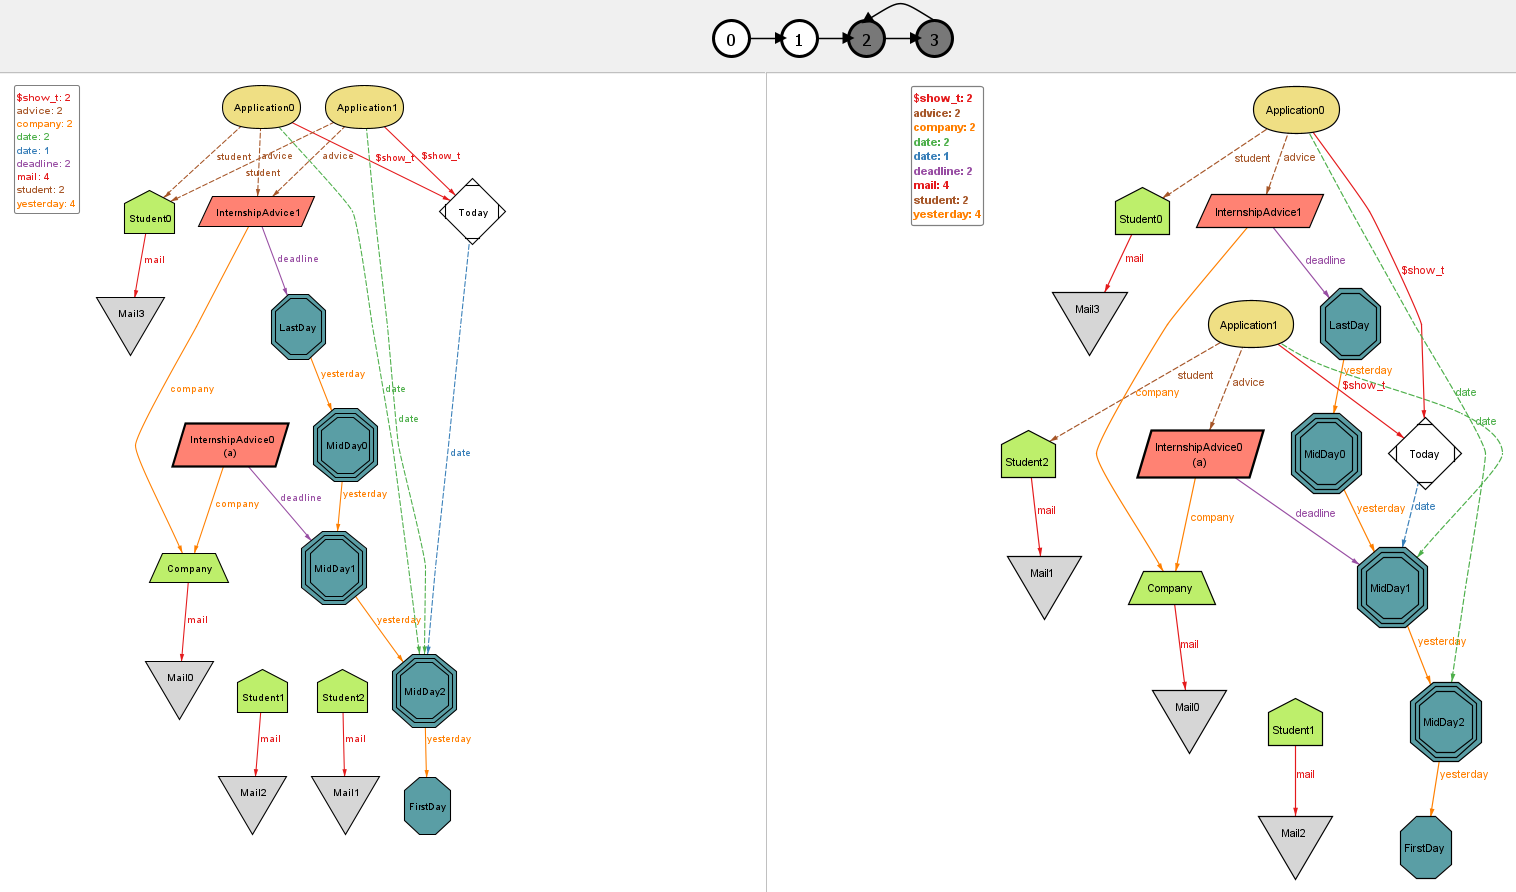
\includegraphics{model1-4.png}
		\end{center}
		\begin{center}
			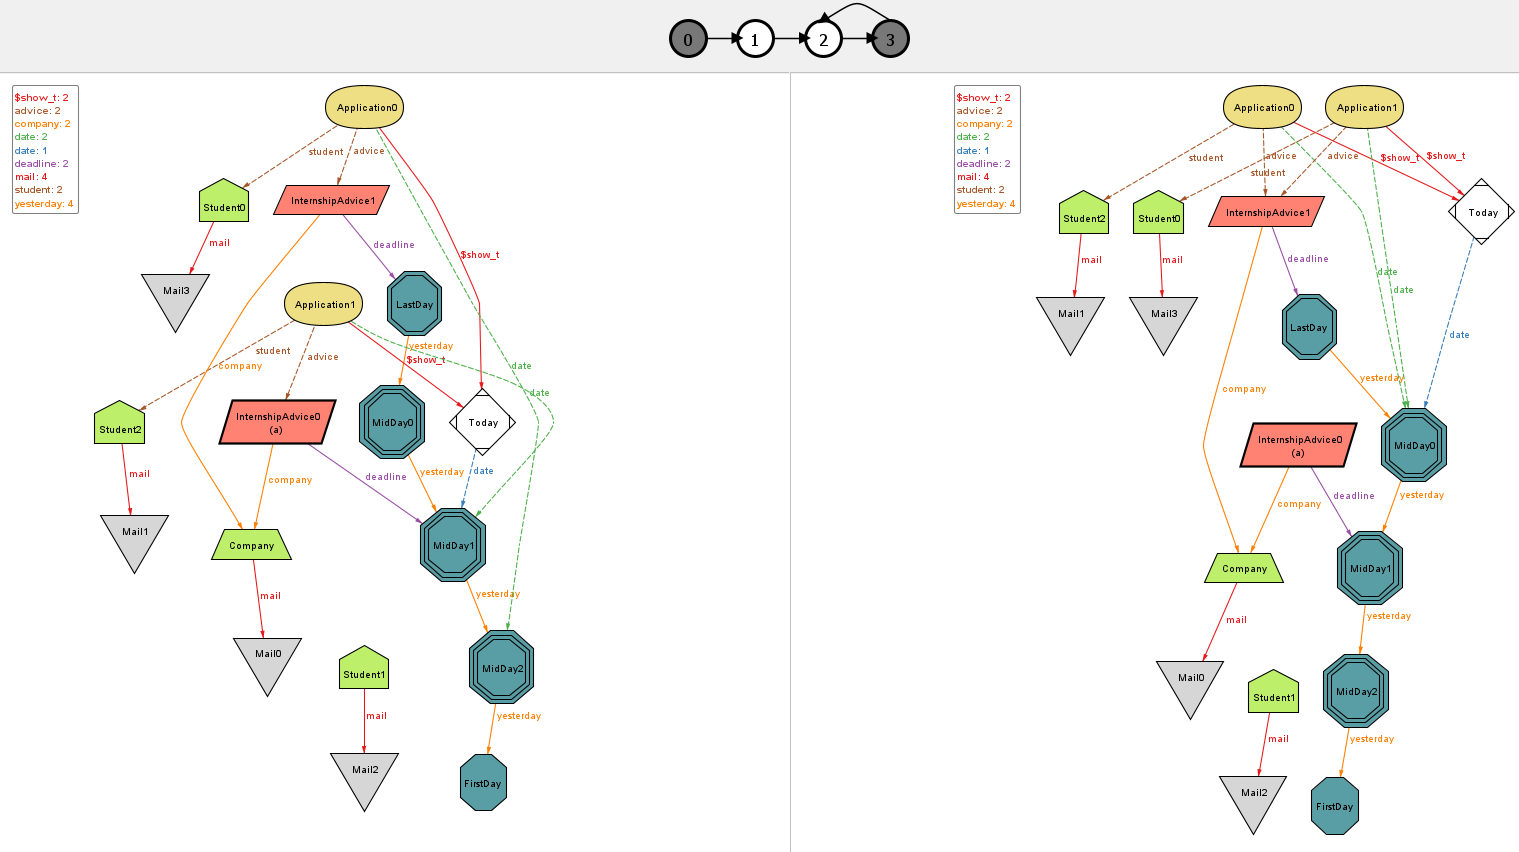
\includegraphics{model1-5.png}
		\end{center}
		\begin{enumerate}[start=0]
			\item the trace starts with two application enrolled \CommentSty{MidDay2} (which is \CommentSty{Today} in this step). These two applications refer to the same \CommentSty{InternshipAdvice} (\CommentSty{InternshipAdvice1});
			\item in this step, \CommentSty{Application0} does not change while \CommentSty{Application1} has its student changed and its advice change. We notice that even the application date is changed to the date point by actual \CommentSty{Today};
			\item in this step each application changes somehow. Their dates are properly updated and they are not related to advice which deadline has already expired.
		\end{enumerate}
		
	\section{Selection process structure (static simulation)}
		Although a selection process has without a doubt a dynamic behavior, we preferred to focus on modeling the constraints related to the process design:
		\begin{center}
			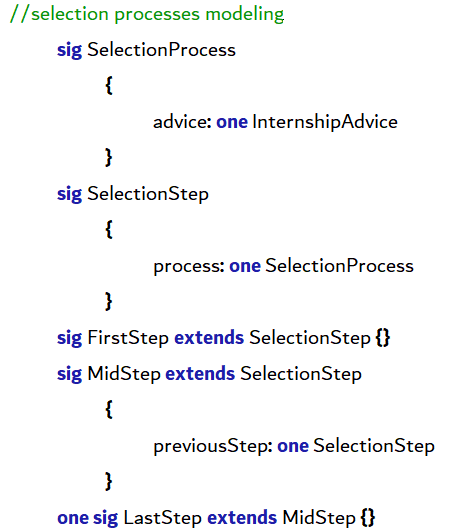
\includegraphics{model2-1.png}
		\end{center}
		\begin{center}
			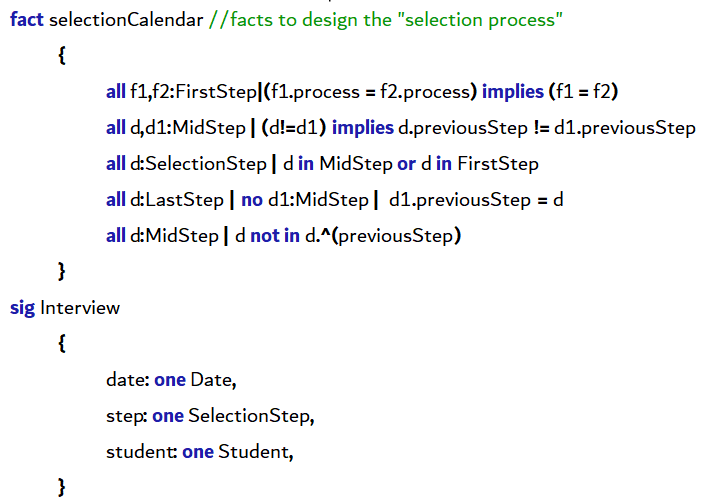
\includegraphics{model2-2.png}
		\end{center}
		\begin{center}
			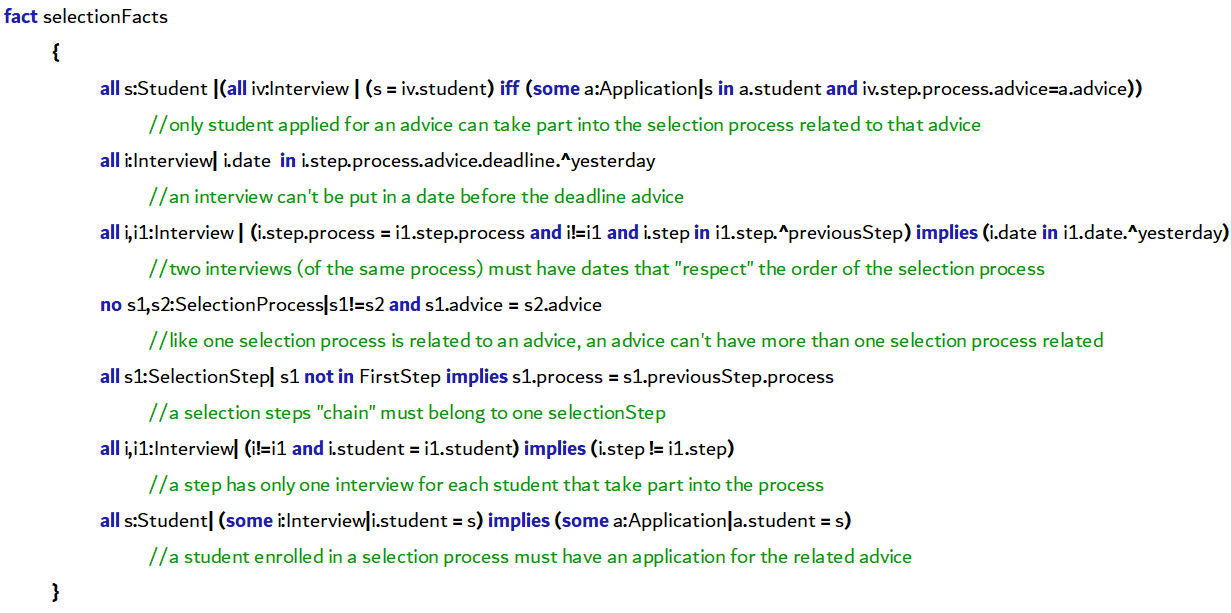
\includegraphics{model2-3.png}
		\end{center}
		These constraints ensure that the process designed by the company does not rise contradictions, such as interviews ordered differently that the related steps.
		Dynamic aspects related to selection processes such as score assignments are generally more interesting from a coherence point of view rather than logical contradictions (e.g. two identical open answers written by two different students should be evaluated in the same way in the context of the same selection process), a part for closed answers.
		\begin{center}
			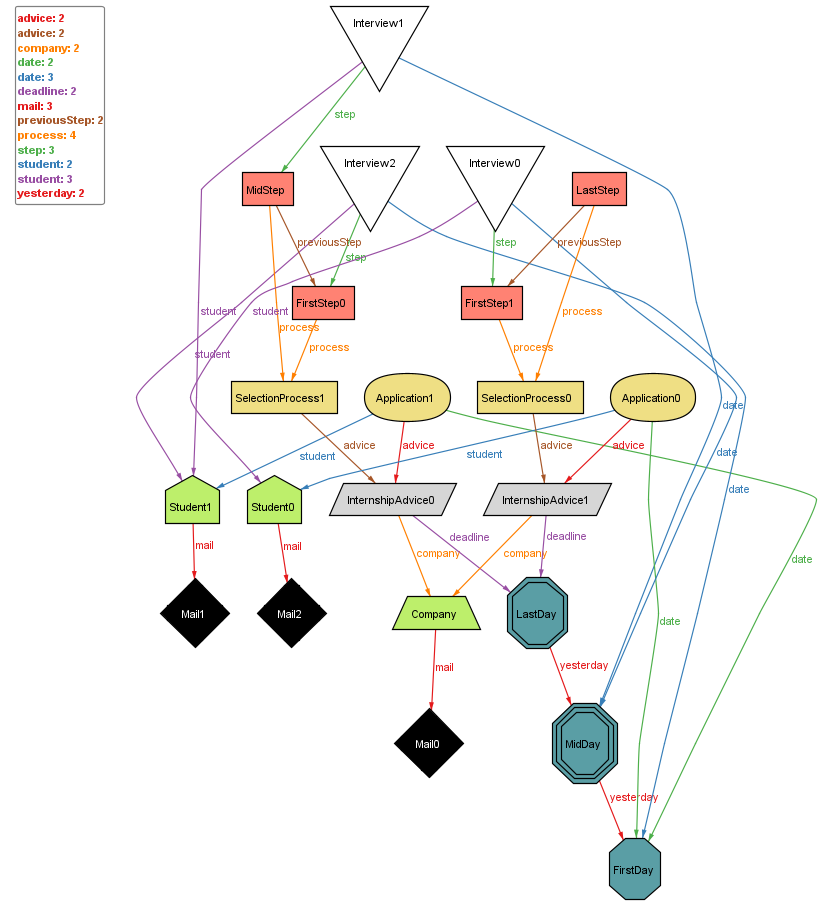
\includegraphics{model2-4.png}
		\end{center}
		At the end, one of the main purposes of this static modeling is also to clarify the selection process structure (also visually).